% (c) Egor Osipov

\documentclass[a4paper,12pt]{article} % тип документа (report, book)
\usepackage[14pt]{extsizes}
\usepackage[left=2cm,right=2cm, top=2cm,bottom=2cm,bindingoffset=0cm]{geometry} % Настройки документа
\usepackage{pgfplots}
\usepackage{pgfplotstable}
\usepackage{tikz} 

%  Русский язык
\usepackage[T2A]{fontenc}			% кодировка
\usepackage[utf8]{inputenc}			% кодировка исходного текста
\usepackage[english,russian]{babel}	% локализация и переносы


% Математика
\usepackage{amsmath,amsfonts,amssymb,amsthm,mathtools} 

% Просто смайлики
\usepackage{wasysym}

%Вставка картинок
\usepackage{graphicx}
\graphicspath{./}
\DeclareGraphicsExtensions{.pdf,.png,.jpg}
\usepackage{float}

% Настройка абзацев
\usepackage{indentfirst}
%\setlength{\parindent}{5ex}
%\setlength{\parskip}{1em}

\begin{document} % начало документа

%Заговолок
\begin{titlepage}
\begin{center}
	\large{Московский физико-технический институт}\\
	\vspace{100px}
	\LARGE{Лабораторная работа № 3.6.1.}\\
	\LARGE{Спектральный анализ электрических сигналов.}\\
	\vspace{30px}
	
\includegraphics[scale = 0.3]{fakt_logo.png}\\
\end{center}

\vfill
\begin{flushright}
	\text{Осипов Егор. Б03-005}\\
	\text{29.10.2021}\\
	\text{г. Долгопрудный}
\end{flushright}
\end{titlepage}

\newpage

\tableofcontents

\newpage

\section{Теория и подготовка к работе.}

\subsection{Цель и приборы, используемые в работе.}

\textbf{Цель работы:} Изучение спектрального состава периодических электрических сигналов.

\textbf{В работе используются:} анализатор спектра, генератор прямоуголных импульсов, генератор сигналов специальной формы, осциллограф.

\subsection{Принцип работы спектроанализатора.}

Для исследования спектров в работе используется гетеродинный анализатор спектра типа СК4-56. Упрощённая структурная схема, поясняющая последовательный супер-гетеродинный метод спектрального анализа внешнего сигнала, изображена на рис \eqref{princip}.

\begin{figure}[H]\label{princip}
	\center{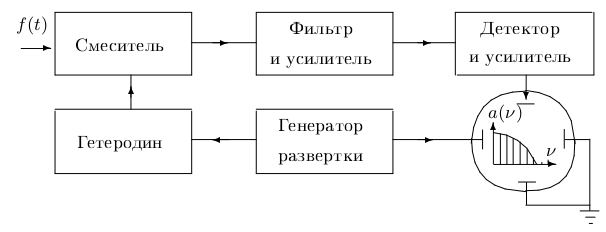
\includegraphics[scale=0.8]{pic1}}
 	\caption{Структурная схема анализатора спектра.}
\label{fig:image2}
\end{figure}

Восстановление спектрального состава входного сигнала $f(x)$ происходит периодически с некоторым заданным периодом. Это время является периодом повторения пилообразного напряжения, которое вырабалывается генератором развёртки. Линейно нарастающее во времени напряжение с генератора развёртки подаётся на гетеродин, который генерирует переменное напряжение с частотой пропорциональной этому напряжению, но с постоянной амплитудой. При изменении пилообразного напряжения от нуля до некоторого максимального значения частота, сигналов, вырабатываемых гетеродином, изменяется в пределах от 128 до 188 кГц. Исследуемый сигнал /(6) и переменное напряжение с гетеродина одновременно поступают на смеситель. При нелинейном сложении этих колебаний на выходе смесителя возникают сигналы суммарной и разностной частоты. Для анализа используется только разностный сигнал. Смешение частот исследуемого сигнала и частоты гетеродина лежит в основе большинства современных радиоприёмных устройств супергетеродинов.

Со смесителя сигнал поступает на фильтр, который настроен на частоту 128 кГц. Таким образом мы «извлекаем» из спектра входного сигнала (6) переменное напряжение с частотой равной разности частот гетеродина и фильтра. За время, равное периоду повторения пилообразкаег колебания с частотами от нуля до 60 кГц. Затем эти колебания детектируются, усиливаются и подаются на вертикальный вход электронно-лучевой трубки (ЭЛТ). Одновременно сигнал с генератора развёртки поступает на горизонтальный вход ЭЛТ. На экране анализатора возникает, таким образом, график, изображающий зависимость амплитуды гармоник от частоты, те. фурье-спектр исследуемого сигнала.

\section{Задание 1. Исследование спектра периодической последовательности прямоугольных испульсов.}

\begin{figure}[H]\label{pic2}
	\center{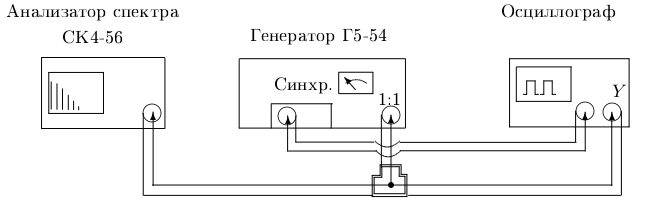
\includegraphics[scale=0.8]{pic2}}
 	\caption{Схема для исследования периодической последовательности прямоугольных испульсов.}
\end{figure}

\subsection{Экспериментальная установка.}

Схема для исследования спектра периодической последовательности прямоугольных импульсов представлена на рис. \eqref{pic2}. Сигнал с выхода генератора прямоугольных импульсов Г5-54 подаётся на вход анализатора спектра и одновременно — на вход \textit{У} осциллографа. С генератора импульсов на осциллограф подабися также сигнал синхронизации, запускающий ждущую развёртку осциллографа. При этом на экране осциллографа можно наблюдать саму последовательность прямоугольных импульсов, а на экране ЭЛТ анализатора спектра — распределение амплитуд спектральных составляющих этой последовательности.

В наблюдаемом спектре отсутствует информация об амилилуде нулевой гармоники, т. е. о величине постоянной составляющей; её местоположение (начало отсчёта шкалы частот) отмечено небольшим вертикальным выбросом.

\subsection{Результаты обработки.}

1. Соберем схему согласно рисунку \eqref{pic2} и подготовим приборы к работе.

2. Установим на анализаторе спектра режим работы с однократной разверсткой и получим на экране спектр импульсов с праметрами $f_\text{повт} = 10^3\text{Гц}$; $\tau = 25 \text{мкс}$; частотыный масштаб $m_x = 5 \text{кГц/дел}$.

Проанализируем, как меняется спектр ($\vartriangle\nu$, $\delta\nu$): 
а) при увеличении $\tau$ вдвое при неизменном $f_\text{повт} = 1 \text{кГц}$; 
б) при увеличении $f_\text{повт}$ вдвое при неизменном $\tau = 25\text{мкс}$.

\begin{figure}[H]\label{pic3}
	\center{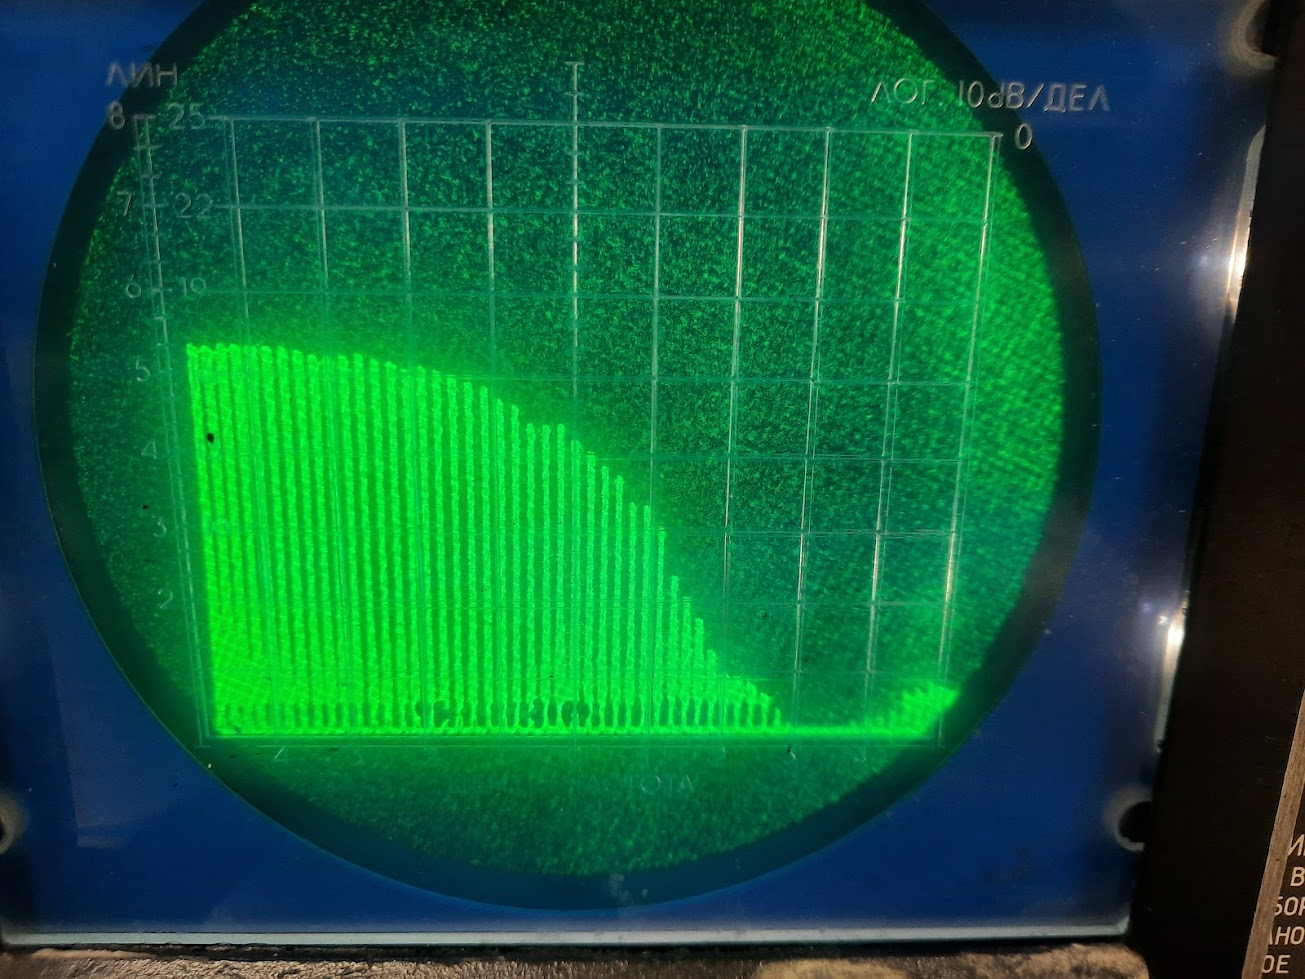
\includegraphics[scale=0.3]{pic3}}
 	\caption{$f_\text{повт} = 10^3\text{Гц}$; $\tau = 25 \text{мкс}$; частотыный масштаб $m_x = 5 \text{кГц/дел}$}
\end{figure}

Из рисунка \eqref{pic3} видно, что $\vartriangle\nu = 7 \text{дел} = 35 \text{кГц}$.

\begin{figure}[H]\label{pic4}
	\center{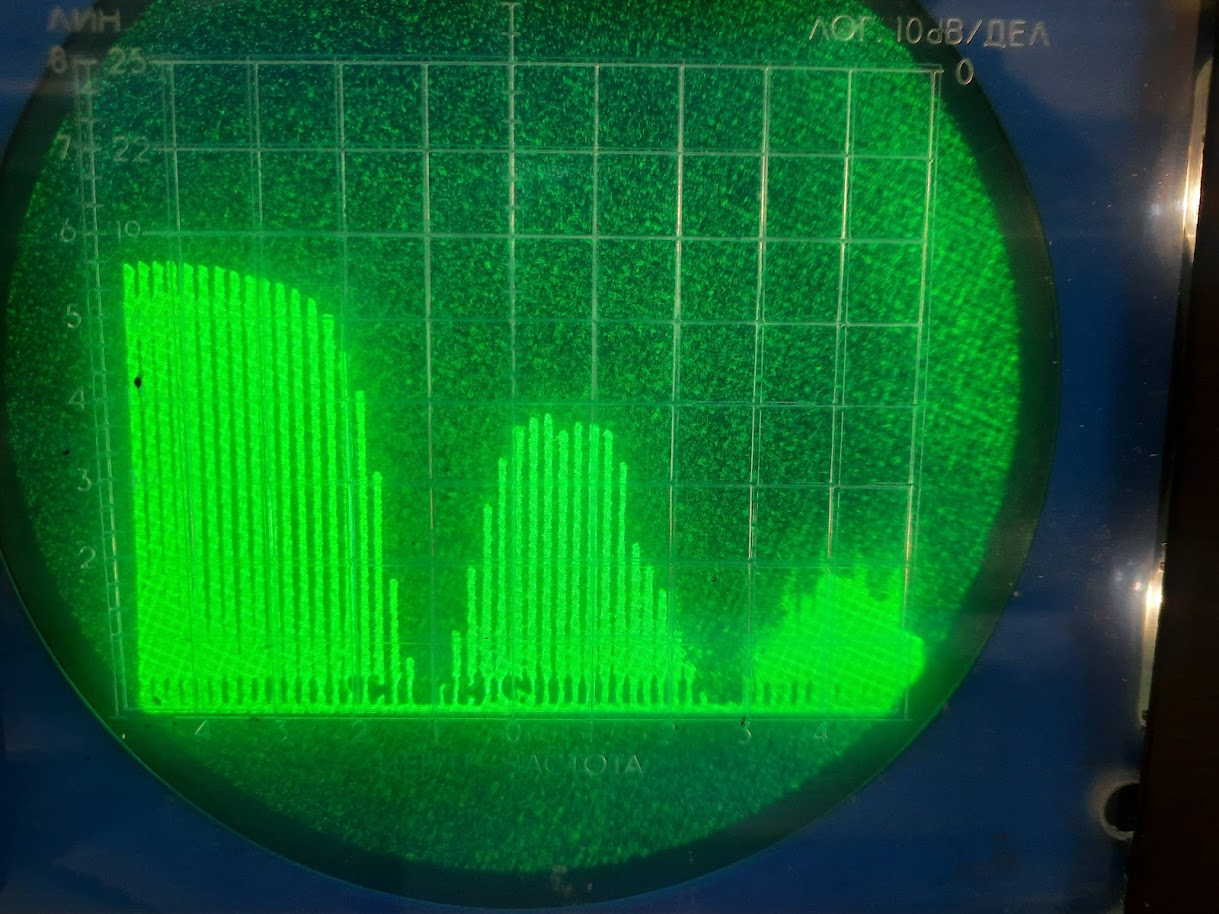
\includegraphics[scale=0.3]{pic4}}
 	\caption{$f_\text{повт} = 10^3\text{Гц}$; $\tau = 50 \text{мкс}$; частотыный масштаб $m_x = 5 \text{кГц/дел}$}
\end{figure}

Из рисунка видно \eqref{pic4}, что $\vartriangle\nu = 3.5 \text{дел} = 17.5 \text{кГц}$.

\begin{figure}[H]\label{pic5}
	\center{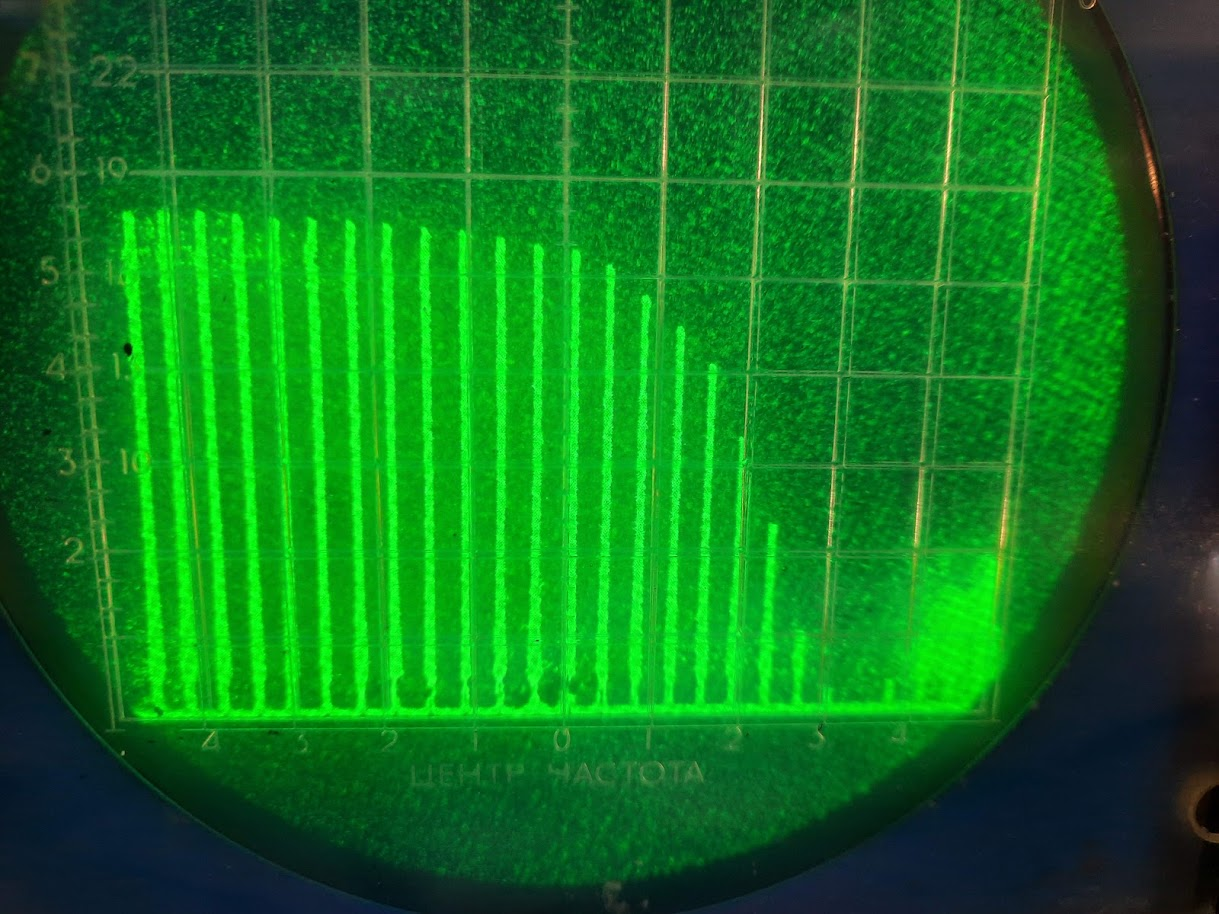
\includegraphics[scale=0.3]{pic5}}
 	\caption{$f_\text{повт} = 2 * 10^3\text{Гц}$; $\tau = 25 \text{мкс}$; частотыный масштаб $m_x = 5 \text{кГц/дел}$}
\end{figure}

Из рисунка видно \eqref{pic5}, что $\vartriangle\nu = 8 \text{дел} = 40 \text{кГц}$.

3. Проведем измерение зависимости ширины спектра от длительности импкльса $\vartriangle\nu(\tau)$ при увеличении $\tau$ от 25 до 200 мкс при $f_\text{повт} = 1 \text{кГц}$. Результаты занесем в таблицу \eqref{tab1}.

\begin{table}[H]
\caption{\label{tab1} Зависимость ширины спектра $\Delta V$ от длительности сигнала $\tau$.}
\begin{center}
\begin{tabular}{|c|c|c|c|c|c|c|c|c|c|}
\hline
$\tau$ & 40 & 60 & 80 & 100 & 120 & 140 & 160 & 180 & 200\\
\hline
$\Delta V$ & 25 & 17 & 12.5 & 10 & 8.3 & 7 & 6.25 & 5.7 & 5\\
\hline
\end{tabular}
\end{center}
\label{table1:ref}
\end{table} 

\begin{center}
\begin{tikzpicture}[baseline]
\begin{axis}[
    title = \text{Зависимость ширины спектра $\Delta V$ от длительности сигнала $\tau$.},
    %legend pos = north west,
    xlabel = {$1/\tau$ мкс $^{-1}$},
    ylabel = {$\Delta V$ кГц},
    width = 0.7\textwidth,
    height = 0.45\textwidth,
    %ymin = 6,
    %ymax = 15,
    %xmin = 4,
    %xmax = 22,
]
\addplot[red, domain = 0.005:0.03] {0.0260498 + 1005.58*x};
\addlegendentry{$y = 1005.58x$};
\addplot[
    red,
    only marks,
    error bars/.cd, y dir=both, y explicit,
] 
table[
    x = X,
    y = Y,
    y error = Ey,
]
{
X   Y   Ey
0.025 25 0.75
0.016666666666666666 17 0.51
0.0125 12.5 0.375
0.01 10 0.3
0.008333333333333333 8.33 0.24989999999999998
0.007142857142857143 7 0.21
0.00625 6.25 0.1875
0.005555555555555556 5.67 0.1701
0.005 5 0.15
};
\end{axis}
\end{tikzpicture}
\end{center}

$\Delta V \cdot \tau = 1.006$, значит, соотношение неопределенности выполняется с точностью 0.6\%.

\begin{table}[H]
\caption{\label{tab2} Характеристики гармоник для $\tau = 50 \mu \text{c}$.}
\begin{center}
\begin{tabular}{|c|c|c|}
\hline
№ Гармоники & Частота (кГц) & Амплитуда (мВ)\\
\hline
1 & 0.063 & 118.1\\
\hline
2 & 1.042 & 69.367\\
\hline
3 & 2.02 & 68.62\\
\hline
4 & 2.998 & 66.42\\
\hline
5 & 4.028 & 63.46\\
\hline
6 & 5.058 & 60.5\\
\hline
7 & 5.985 & 56.08\\
\hline
8 & 7.015 & 51.65\\
\hline
9 & 7.942 & 47.96\\
\hline
10 & 8.972 & 43.53\\
\hline
11 & 10.05 & 40.58\\
\hline
12 & 12.01 & 33.2\\
\hline
13 & 12.06 & 32.47\\
\hline
14 & 12.99 & 29.51\\
\hline
15 & 14.02 & 24.35\\
\hline
16 & 15.0 & 19.92\\
\hline
17 & 15.97 & 15.5\\
\hline
18 & 17.0 & 11.87\\
\hline
19 & 18.03 & 7.379\\
\hline
\end{tabular}
\end{center}
\label{table1:ref}
\end{table}

\begin{figure}[H]\label{pic6}
	\center{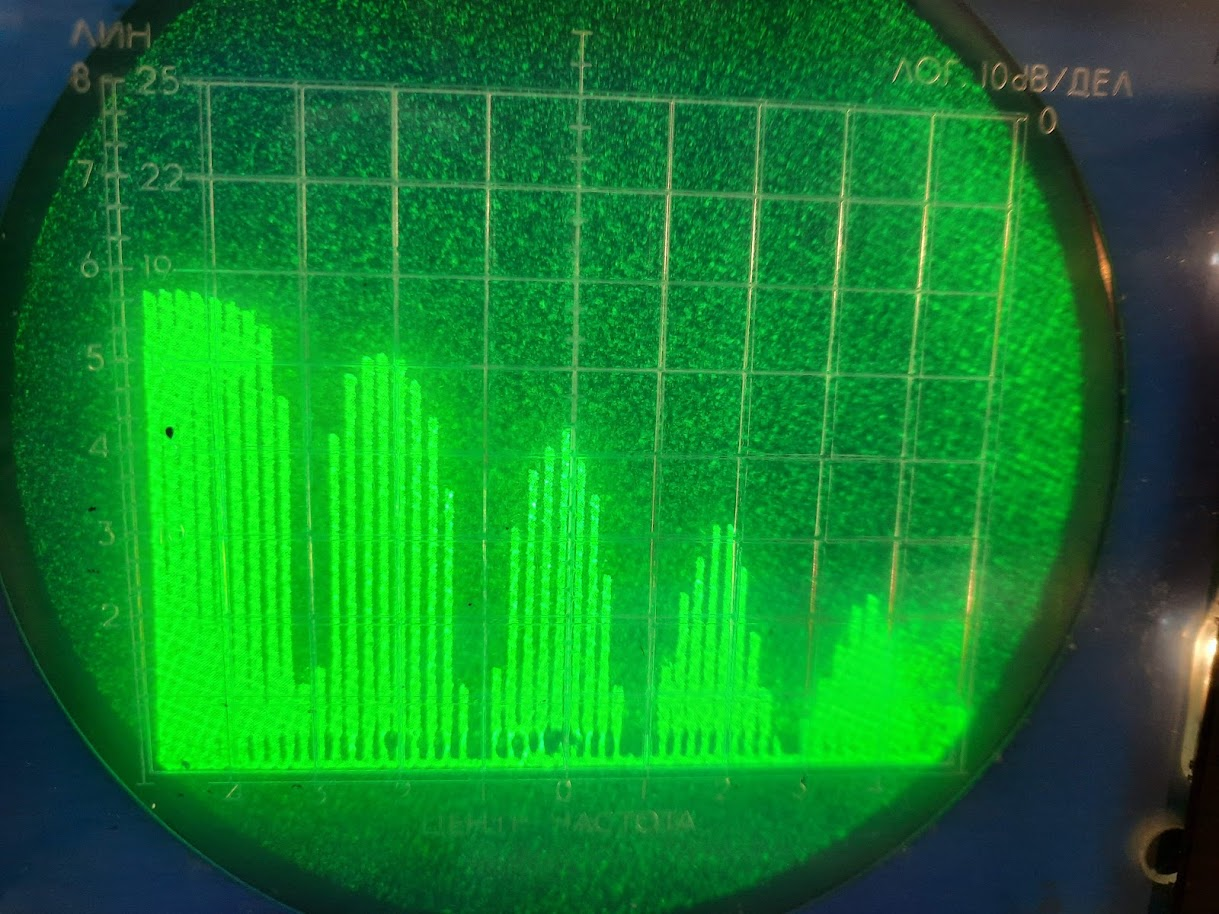
\includegraphics[scale=0.3]{pic6}}
 	\caption{Спектр для $f_\text{повт} = 10^3\text{Гц}$; $\tau = 100 \text{мкс}$; частотыный масштаб $m_x = 5 \text{кГц/дел}$}
\end{figure}

\begin{table}[H]
\caption{\label{tab3} Характеристики гармоник для $\tau = 100 \mu \text{c}$.}
\begin{center}
\begin{tabular}{|c|c|c|}
\hline
№ Гармоники & Частота (кГц) & Амплитуда (мВ)\\
\hline
1 & 0.063 & 219.1\\
\hline
2 & 0.99 & 137.2\\
\hline
3 & 2.02 & 129.1\\
\hline
4 & 2.998 & 118.8\\
\hline
5 & 4.028 & 103.3\\
\hline
6 & 5.058 & 86.33\\
\hline
7 & 6.036 & 65.67\\
\hline
8 & 7.066 & 46.49\\
\hline
9 & 7.993 & 29.51\\
\hline
10 & 9.075 & 13.28\\
\hline
\end{tabular}
\end{center}
\label{tab3}
\end{table}

\section{Задание 2. Исследование спектра периодической последовательности цугов гармонических колебаний.}

\subsection{Экспериментальная установка.}

Экспериментальная установка. Исследование спектра периодически чередующихся цугов гармонических колебаний проводится по схеме, изображённой на рис. \eqref{pic7}. Генератор Г6-З4 вырабатывает синусоидальные колебания высокой частоты. На вход АМ (амилитудная модуляция) этого генератора подаются прямоугольные импульсы с генералора Г5-54, а на выходе мы получаем высокочастотные модулированные колебания в виде отдельных кусков синусоиды — цугов. Эти пуги с выхода генератора Г6-34 поступают на вход спектроанализатора и одновременно на вход У осциллографа. Сигнал синхронизации подавтся на вход Х осциллографа с генератора импульсов.

\begin{figure}[H]\label{pic7}
	\center{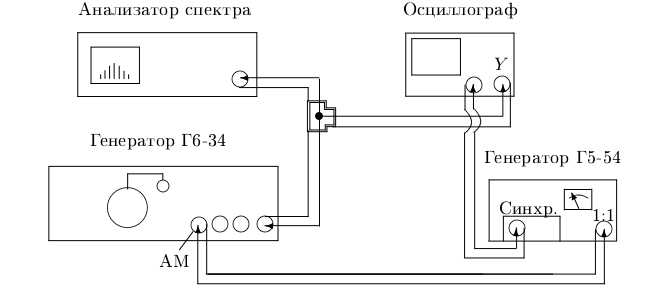
\includegraphics[scale=0.8]{pic7}}
 	\caption{Схема для исследования спектра периодической последовательности цугов высокочастотных колебаний.}
\end{figure}

\subsection{Результаты обработки.}

1. Соберем схему изображеннцю на рисунке \eqref{pic7} и подготовим приборы к работе.

2. Установим частоту несущей $\nu_0 = 25\text{кГц}$ и проанализируем, как меняется вид спектра: а) при увеличении длительности импульса вдвое ($\tau = 50\text{, } 100 \text{мкс}$ для $f_\text{повт} = 1 \text{кГц}$); б) при измерении частоты несущей: $\nu_0 = 25 \text{, } 10 \text{ или } 40 \text{ кГц}$.

\begin{figure}[H]\label{pic8}
	\center{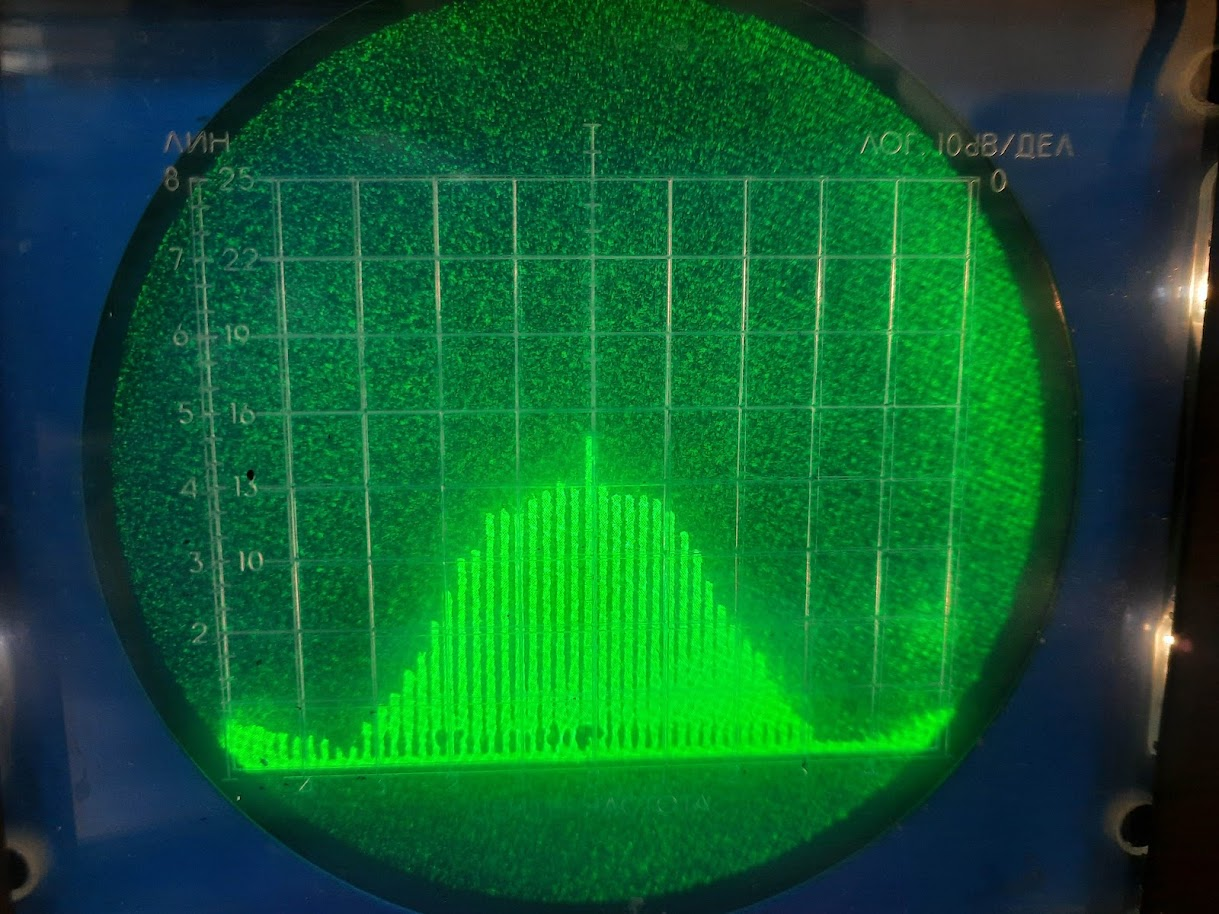
\includegraphics[scale=0.3]{pic8}}
 	\caption{При $\nu_0 = 25 \text{кГц}$}
\end{figure}

3. При фиксированной длительности импульсов $\tau = 50 \text{мкс}$ исследуем зависимость расстояния $\delta \nu$ от между соседними спектральными компонентами от периода T (частыт повторения импульсов $f_\text{повт}$ в диапазоне от 1 до 8 кГц).

\begin{table}[H]
\caption{\label{tab4} Зависимость расстояния между соседними спектральными компонентами $\delta \nu$ от частоты повторения импульсов $f_\text{повт.}$.}
\begin{center}
\begin{tabular}{|c|c|c|c|c|c|c|}
\hline
$f_\text{повт.}$ & 0.5 & 1 & 2 & 3 & 4 & 5\\
\hline
$\delta \nu$ & 0.5 & 1 & 2 & 3 & 4 & 5\\
\hline
\end{tabular}
\end{center}
\label{tab4}
\end{table}

Зависимость $\delta \nu$ от $f_\text{повт.}$ полностью совпадает с теоритической: угловой коэффициент равен 1.

\section{Исследование спектра гармонических сигналов модулированных по амплитуде}

\subsection{Экспериментальная установка.}

Схема для исследования амплитудно-модулированного сигнала представлена на рис. \eqref{pic9}. Модуляционный генератор встроен в левую часть генератора сигналов Гб-34 . Синусоидальный сигнал с частотой модуляции $f_\text{мод}$ = 1 кГц подается с модуляционного генератора на вход АМ (амилитудная модуляция) генератора, вырабатывающего синусоидальный сигнал высокой частоты (частота несущей $ \nu_0 = 25 \text{кГц}$). Амплитудно-модулированный сигнал с основного выхода генератора поступает на осциллограф и на анализатор спектра.

\begin{figure}[H]\label{pic9}
	\center{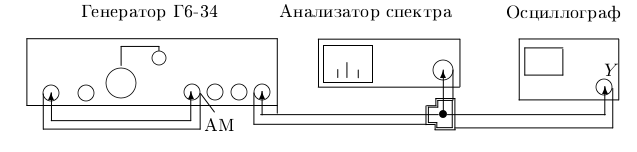
\includegraphics[scale=0.8]{pic9}}
 	\caption{Схема для исследования спектра высокочастотного гармонического сигнала, промодулированного по амплитуде низкочастотным гармоническим сигналом.}
\end{figure}

\subsection{Обработка результатов.}

1. Соберем установку по схеме \eqref{pic9}, подготовим приборы к использованию.

2. Измеряя глубину модуляции, исследуем зависимость отношения амплитуды боковой линии спектра к амплитуде основной линии от глубины модуляции m; для рассчеты глубины модуляции m воспользуемся формулой 6.13, измеряя максимальную $2A_\text{max}$ и минимальную $2A_\text{min}$ амплитуды сигнала на экране осциллографа.

3. Построим график отнощения амплитуды боковой линии спектра к амплитуде основной линии от глубины модуляции m. Определим угол наклона графика и сравним с рассчетным по формуле 6.14.

\begin{figure}[H]\label{pic10}
	\center{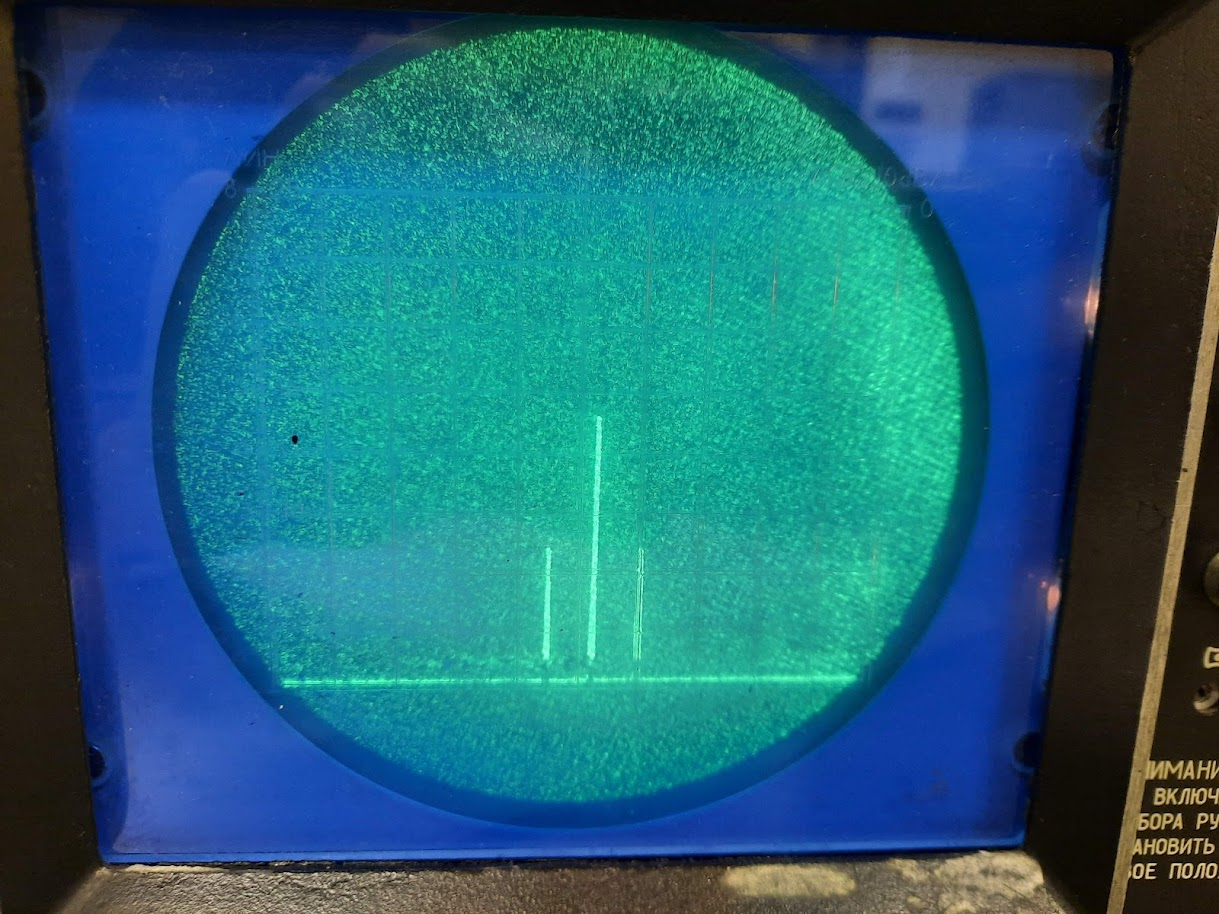
\includegraphics[scale=0.3]{pic10}}
 	\caption{Пример изображения амплитуд боковых линий спектра и основной линии.}
\end{figure}

\begin{table}[H]
\caption{\label{tab:canonsummary} Амплитудные характеристики.}
\begin{center}
\begin{tabular}{|c|c|c|c|c|c|c|c|}
\hline
Амплитуда (мВ) & 0.2 & 1 & 1.5 & 2\\
\hline
$A_{min}$ (мВ) & 441.7 & 240.6 & 125.7 & 16.44\\
\hline
$A_{max}$ (мВ) & 542.2 & 750.4 & 872.5 & 991.5\\
\hline
$a_\text{осн}$ (мВ) & 324.7 & 324.7 & 324.7 & 317.2\\
\hline
$a_\text{бок}$ (мВ) & 15.67 & 81.36 & 120.2 & 156.7\\
\hline
$m$ & 0.102 & 0.514 & 0.748 & 0.967\\
\hline
\end{tabular}
\end{center}
\label{table1:ref}
\end{table}

\begin{center}
\begin{tikzpicture}[baseline]
\begin{axis}[
    title = \text{Зависимость отношения $a_\text{бок}$ к $a_\text{осн}$ от глубины модуляции m.},
    legend pos = north west,
    xlabel = {m},
    ylabel = {$a_\text{бок}$ / $a_\text{осн}$},
    width = 0.7\textwidth,
    height = 0.45\textwidth,
    %ymin = 6,
    %ymax = 15,
    %xmin = 4,
    %xmax = 22,
]
\addplot[red, domain = 0.1:1] {-0.00329361 + 0.497463*x};
\addlegendentry{$y = 0.497x$};
\addplot[
    red,
    only marks,
    error bars/.cd, y dir=both, y explicit,
] 
table[
    x = X,
    y = Y,
    y error = Ey,
]
{
X   Y   Ey
0.10214452688281334 0.04825993224514937 0.001447797967354481
0.5144298688193744 0.2505697566984909 0.007517092700954727
0.7481466639951913 0.37018786572220513 0.011105635971666153
0.967379010655396 0.49401008827238335 0.0148203026481715
};
\end{axis}
\end{tikzpicture}
\end{center}

Коэффициент наклона, равный 0.497, отличается от рассчитаггого теоретически на 0.6\%

\section{Вывод}
Исследован спектр сигнала переодической последовательности прямоугольных импульсов, переодической последовательности цугов и сигнала, промодулированного по амплитуде. Установлены качественные изменения картин спектров при изменении параметров колебаний.

\end{document} % конец документа